% ============================================================
%  GeoMetric — Multi-Map Spatial Analytics Portfolio
%  Author    : Muhammad Nouman Hafeez
%  Institute : FAST-NUCES, Islamabad
%  Date      : March 2026
%  Compiler  : pdflatex — run TWICE for TOC and cross-refs
%
%  FOLDER LAYOUT ASSUMED:
%    report/
%      GeoMetric_Report_Final.tex   <- this file
%    outputs/
%      figures/
%        part1_projections/
%        part2_choropleth/
%        ...
% ============================================================

\documentclass[12pt, a4paper, oneside]{report}

% ── Encoding & fonts ─────────────────────────────────────────
\usepackage[T1]{fontenc}
\usepackage[utf8]{inputenc}
\usepackage{lmodern}
\usepackage{microtype}

% ── Page geometry ────────────────────────────────────────────
% A4 = 210mm wide; left=30mm right=25mm => textwidth = 155mm = 15.5cm
\usepackage[
  a4paper,
  top=2.5cm, bottom=2.5cm,
  left=3.0cm, right=2.5cm,
  headheight=24.02pt
]{geometry}

% ── Colours ──────────────────────────────────────────────────
\usepackage[dvipsnames, table]{xcolor}
%   table option also loads colortbl, enabling \rowcolor in tables
\definecolor{primary}{RGB}{26,60,100}
\definecolor{accent}{RGB}{0,130,160}
\definecolor{lightgray}{RGB}{245,245,245}
\definecolor{linkblue}{RGB}{0,90,160}

% ── Graphics ─────────────────────────────────────────────────
\usepackage{graphicx}
\graphicspath{
  {../outputs/figures/}%   when compiling from report/
  {outputs/figures/}%      when compiling from repo root
  {./}%                    fallback: PNGs in same folder as .tex
}
\usepackage{float}
\usepackage{caption}
\usepackage{subcaption}

% ── Tables: array/tabularx loaded *after* parskip (see below) ──

% ── Mathematics ──────────────────────────────────────────────
\usepackage{amsmath,amssymb}

% ── Code / verbatim ──────────────────────────────────────────
\usepackage{listings}
\usepackage{fancyvrb}
\lstset{
  basicstyle       = \ttfamily\footnotesize,
  backgroundcolor  = \color{lightgray},
  frame            = single,
  framerule        = 0pt,
  breaklines       = true,
  breakatwhitespace= true,
  columns          = fullflexible,
  captionpos       = b,
  keywordstyle     = \color{accent}\bfseries,
  commentstyle     = \color{gray}\itshape,
  stringstyle      = \color{primary},
  numbers          = left,
  numberstyle      = \tiny\color{gray},
  numbersep        = 8pt,
  showstringspaces = false,
  tabsize          = 4,
  xleftmargin      = 12pt,
  xrightmargin     = 4pt,
}

% ── Headers & footers ────────────────────────────────────────
\usepackage{fancyhdr}
\pagestyle{fancy}
\fancyhf{}
\fancyhead[L]{\small\color{primary}\textit{GeoMetric: Multi-Map Spatial Analytics}}
\fancyhead[R]{\small\color{primary}\textit{Muhammad Nouman Hafeez}}
\fancyfoot[C]{\small\color{gray}---\;\thepage\;---}
\renewcommand{\headrulewidth}{0.4pt}
\renewcommand{\headrule}{%
  \hbox to\headwidth{\color{accent}\leaders\hrule height\headrulewidth\hfill}}
\renewcommand{\footrulewidth}{0pt}
\fancypagestyle{plain}{%
  \fancyhf{}%
  \fancyfoot[C]{\small\color{gray}---\;\thepage\;---}%
  \renewcommand{\headrulewidth}{0pt}%
}

% ── Chapter / section headings ───────────────────────────────
\usepackage{titlesec}
\titleformat{\chapter}[display]
  {\normalfont\huge\bfseries\color{primary}}
  {\color{accent}\chaptertitlename~\thechapter}{12pt}{\Huge}
\titlespacing*{\chapter}{0pt}{10pt}{20pt}
\titleformat{\section}
  {\normalfont\Large\bfseries\color{primary}}
  {\color{accent}\thesection}{1em}{}
\titlespacing*{\section}{0pt}{14pt}{6pt}
\titleformat{\subsection}
  {\normalfont\large\bfseries\color{primary!80}}
  {\thesubsection}{1em}{}
\titlespacing*{\subsection}{0pt}{10pt}{4pt}

% ── Hyperlinks (always load near last) ───────────────────────
\usepackage[
  colorlinks  = true,
  linkcolor   = linkblue,
  urlcolor    = accent,
  citecolor   = primary,
  bookmarks   = true,
  bookmarksopen = true,
  pdfauthor   = {Muhammad Nouman Hafeez},
  pdftitle    = {GeoMetric: From Raw Spatial Data to Insightful Maps},
  pdfsubject  = {Multi-Map Spatial Analytics in Python},
  pdfkeywords = {GeoPandas choropleth projections flow-map cartogram}
]{hyperref}
\usepackage{xurl}
\renewcommand{\UrlFont}{\ttfamily}
\usepackage{bookmark}

% ── Miscellaneous ────────────────────────────────────────────
\usepackage{enumitem}
\usepackage{setspace}
\usepackage{parskip}
% Tables: load after parskip so colortbl + older array do not leave \insert@pcolumn undefined
\usepackage{booktabs}
\usepackage{multirow}
\usepackage{array}
\newcolumntype{L}[1]{>{\raggedright\arraybackslash}p{#1}}
\newcolumntype{C}[1]{>{\centering\arraybackslash}p{#1}}
\newcolumntype{R}[1]{>{\raggedleft\arraybackslash}p{#1}}
\newcolumntype{Z}{>{\raggedright\arraybackslash}X}
\makeatletter
\@ifundefined{insert@pcolumn}{\let\insert@pcolumn\insert@column}{}
\makeatother
\usepackage{tabularx}
\usepackage{longtable}
\usepackage{pifont}
\usepackage{fontawesome5}   % provides \faMap \faSitemap \faChartBar etc.
\usepackage{tcolorbox}
\tcbuselibrary{breakable,skins}
\usepackage{tikz}
\usetikzlibrary{shapes,arrows.meta,positioning}

% ── Custom tcolorbox environments ────────────────────────────
\newtcolorbox{infobox}[1][]{
  enhanced, breakable,
  colback=accent!8, colframe=accent,
  boxrule=0.6pt, arc=3pt,
  title={#1},
  fonttitle=\bfseries\color{white},
  coltitle=white,
  attach boxed title to top left={yshift=-2mm,xshift=4mm},
  boxed title style={colback=accent,arc=2pt},
}
\newtcolorbox{limitbox}{
  enhanced,
  colback=orange!8, colframe=orange!70!black,
  boxrule=0.6pt, arc=3pt, leftrule=4pt,
}
\newtcolorbox{designbox}{
  enhanced,
  colback=primary!5, colframe=primary,
  boxrule=0.6pt, arc=3pt, leftrule=4pt,
}

% ── Caption style ────────────────────────────────────────────
\captionsetup{
  font=small,
  labelfont={bf,color=primary},
  textfont=it,
  margin=10pt,
  belowskip=4pt,
}

% ── Global line spacing ──────────────────────────────────────
\setstretch{1.2}

% ── Convenience macro: consistent table row height ───────────
\newcommand{\ts}{\renewcommand{\arraystretch}{1.35}}

% =============================================================
\begin{document}
% =============================================================

% ─────────────────────────────────────────────────────────────
%  COVER PAGE
% ─────────────────────────────────────────────────────────────
\begin{titlepage}
  \thispagestyle{empty}
  \pagecolor{primary}

  \begin{tikzpicture}[remember picture,overlay]
    \fill[accent]          (current page.north west)
      rectangle ([yshift=-1.8cm]current page.north east);
    \fill[white!20!accent] (current page.south west)
      rectangle ([yshift=2cm]current page.south east);
  \end{tikzpicture}

  \vspace*{1.6cm}
  \begin{center}

    {\color{white!70!gray}\large\scshape
      FAST-NUCES, Islamabad \quad$\bullet$\quad March 2026}

    \vspace{1.2cm}
    {\color{white}\fontsize{40}{50}\selectfont\bfseries GeoMetric}

    \vspace{0.5cm}
    {\color{accent!60!white}\rule{0.62\textwidth}{0.8pt}}

    \vspace{0.5cm}
    {\color{white!90!gray}\LARGE\itshape
      From Raw Spatial Data to Insightful Maps}

    \vspace{0.3cm}
    {\color{white!70!gray}\large
      Multi-Map Spatial Analytics in Python}

    \vspace{1.8cm}

    % Icon badges — written out explicitly (no \foreach needed)
    \begin{tabular}{@{}ccc@{}}
      \textcolor{accent!80!white}{\Large\faMap}       &
      \textcolor{accent!80!white}{\Large\faSitemap}   &
      \textcolor{accent!80!white}{\Large\faChartBar}  \\[5pt]
      \textcolor{white!80!gray}{\small Projections}   &
      \textcolor{white!80!gray}{\small Flow Maps}     &
      \textcolor{white!80!gray}{\small Choropleths}   \\
    \end{tabular}

    \vspace{1.2cm}
    {\color{accent!60!white}\rule{0.48\textwidth}{0.4pt}}

    \vspace{1.0cm}
    {\color{white}\Large\bfseries Muhammad Nouman Hafeez}

    \vspace{0.4cm}
    {\color{white!70!gray}\normalsize
      BS Computer Science \quad$|$\quad Spatial Computing \& GIS}

    \vspace{0.6cm}
    {\color{white!60!gray}\small
      Department of Computer Science\\[3pt]
      FAST National University of Computer and Emerging Sciences\\[3pt]
      Islamabad, Pakistan}

    \vspace{1.8cm}

    % Tech-stack badges — explicit list, no \foreach
    \fcolorbox{accent!70!white}{accent!15!primary}{%
      \textcolor{white!90!gray}{\small\ttfamily GeoPandas}}\hspace{3pt}%
    \fcolorbox{accent!70!white}{accent!15!primary}{%
      \textcolor{white!90!gray}{\small\ttfamily Matplotlib}}\hspace{3pt}%
    \fcolorbox{accent!70!white}{accent!15!primary}{%
      \textcolor{white!90!gray}{\small\ttfamily mapclassify}}\hspace{3pt}%
    \fcolorbox{accent!70!white}{accent!15!primary}{%
      \textcolor{white!90!gray}{\small\ttfamily Folium}}\hspace{3pt}%
    \fcolorbox{accent!70!white}{accent!15!primary}{%
      \textcolor{white!90!gray}{\small\ttfamily Plotly}}\hspace{3pt}%
    \fcolorbox{accent!70!white}{accent!15!primary}{%
      \textcolor{white!90!gray}{\small\ttfamily NetworkX}}\hspace{3pt}%
    \fcolorbox{accent!70!white}{accent!15!primary}{%
      \textcolor{white!90!gray}{\small\ttfamily SciPy}}\hspace{3pt}%
    \fcolorbox{accent!70!white}{accent!15!primary}{%
      \textcolor{white!90!gray}{\small\ttfamily PySAL}}%

  \end{center}

  \vfill
  {\color{white!50!gray}\footnotesize\centering
    Submitted in partial fulfilment of the Data Visualization coursework requirements.\\[2pt]
    All maps generated at 300\,DPI\@; interactive HTML exports via Folium and Plotly.}
\end{titlepage}

\nopagecolor   % restore white background after cover

% ─────────────────────────────────────────────────────────────
%  ABSTRACT
% ─────────────────────────────────────────────────────────────
\clearpage
\thispagestyle{plain}
\chapter*{Abstract}
\addcontentsline{toc}{chapter}{Abstract}

\begin{infobox}[Executive Summary]
This report documents a fully reproducible Python workflow for global climate and mobility
mapping. Multiple real-world datasets are loaded, cleaned, and spatially joined; seven
analytical parts cover \textbf{coordinate reference system projections},
\textbf{choropleth classification}, \textbf{proportional symbols},
\textbf{airline flow analysis}, \textbf{continuous-field interpolation},
\textbf{cartogram construction}, and \textbf{scenario-based map design}.
Optional interactive exports (Folium, Plotly Dash) and spatial autocorrelation
statistics (Moran's\,I, LISA) extend the core deliverables. Design choices and
known limitations are recorded for every map type in companion text files.
\end{infobox}

\vspace{0.8em}
The portfolio demonstrates that \emph{map choice and classification} shape analytical
narrative as powerfully as the underlying data. By working through the full pipeline ---
from raw CSV and GeoJSON downloads to polished 300\,DPI figures --- this project builds
practical fluency in the complete geospatial analysis stack.

\bigskip
\noindent\textbf{Keywords:} coordinate projections, choropleth mapping, proportional
symbols, flow maps, IDW/RBF interpolation, Dorling cartogram, spatial autocorrelation,
GeoPandas, Matplotlib, Folium.

% ─────────────────────────────────────────────────────────────
%  FRONT MATTER
% ─────────────────────────────────────────────────────────────
\clearpage
\tableofcontents

\clearpage
\listoffigures
\addcontentsline{toc}{chapter}{List of Figures}

\listoftables
\addcontentsline{toc}{chapter}{List of Tables}

% =============================================================
\chapter{Introduction}
% =============================================================

Geospatial analysis rests on a fundamental principle: \textbf{the map type must match the
analytical question}. A choropleth encoding raw population counts misleads the reader
differently from one showing population density; a flow map without magnitude filtering
buries dominant corridors in visual noise. This portfolio implements the complete analytical
pipeline --- from source data through reproducible Python scripts to publication-quality
figures --- demonstrating that every cartographic decision carries epistemic weight.

\section{Project Objectives}

\begin{enumerate}[leftmargin=2em, label=\textcolor{accent}{\bfseries\arabic*.}]
  \item Acquire, document, and version-control at least four distinct spatial dataset
        categories: polygons, points, flows, and a continuous field.
  \item Construct a reproducible, configuration-driven pipeline using
        \texttt{run\_all.py} so that every figure regenerates from a single command.
  \item Produce seven analytically distinct map products, each with a documented
        design rationale and a written limitations statement.
  \item Extend the core pipeline with interactive HTML exports and optional spatial
        statistics (Moran's\,I / LISA).
\end{enumerate}

\section{Technical Stack}

\ts
\begin{table}[H]
  \centering
  \caption{Core Python libraries and their roles in the pipeline.}
  \label{tab:stack}
  \begin{tabularx}{\textwidth}{@{} L{2.5cm} >{\centering\arraybackslash}p{1.4cm} Z @{}}
    \toprule
    \textbf{Library} & \textbf{Min.\ ver.} & \textbf{Role in pipeline} \\
    \midrule
    GeoPandas        & 0.14   & Spatial data I/O, attribute and spatial joins, reprojection \\
    Matplotlib       & 3.8    & Static figure rendering at 300\,DPI \\
    mapclassify      & 2.6    & Choropleth classification (quantile, Jenks, equal interval) \\
    Folium           & 0.15   & Interactive HTML maps with Leaflet backend \\
    Plotly / Dash    & 5.x / 2.x & Animated temporal choropleths and interactive dashboard \\
    SciPy            & 1.12   & RBF and IDW spatial interpolation \\
    NetworkX         & 3.2    & Directed graph, hub and centrality metrics \\
    PySAL (optional) & 23.x   & Global Moran's\,I and LISA spatial autocorrelation \\
    \bottomrule
  \end{tabularx}
\end{table}

\section{Minimum Technical Requirements}

All of the following requirements are satisfied and evidenced throughout this report:

\begin{itemize}[leftmargin=2em, label=\textcolor{accent}{\ding{52}}]
  \item Multiple spatial datasets across all four geometry categories
  \item Attribute and spatial joins across datasets
  \item Both polygon and point geometry types
  \item Repeated reprojection across all seven parts
  \item Six or more analytically distinct map products
  \item Legends, source notes, and scale indicators on every figure
  \item Documented limitations per map type
\end{itemize}

\section{Repository Structure}

\begin{figure}[H]
  \centering
  \begin{BVerbatim}[fontsize=\small]
GeoMetric/
+-- data/
|   +-- raw/               downloaded source files (git-ignored)
|   `-- processed/         GeoPackages and cleaned CSVs
+-- scripts/
|   +-- utils/             config.py  data_loader.py  preprocess.py
|   +-- parts/             part1_projections.py ... part7_scenarios.py
|   `-- bonus/             bonus_dashboard.py  bonus_animation.py
+-- outputs/
|   +-- figures/           PNG maps (300 DPI default)
|   `-- interactive/       Folium HTML, Plotly HTML, animations
+-- notebooks/             one Jupyter notebook per part
+-- webapp/                optional static gallery
+-- docs/                  WORKFLOW.md  dataset_inventory.md
+-- report/                this document + BUILD_PDF.md
+-- tests/                 pytest suite
+-- run_all.py             pipeline entry-point
`-- requirements.txt
  \end{BVerbatim}
  \caption{Top-level directory layout of the GeoMetric repository.}
  \label{fig:repolayout}
\end{figure}

% =============================================================
\chapter{Part~0 --- Dataset Collection and Documentation}
% =============================================================

The pipeline ingests five primary sources covering the four required geometry categories.
Table~\ref{tab:datasets} provides the complete inventory.

\section{Dataset Inventory}

\small
\ts
\setlength{\tabcolsep}{4pt}
\begin{longtable}{@{}
    L{2.2cm}
    L{1.7cm}
    L{1.7cm}
    C{1.3cm}
    L{7.2cm}
  @{}}
  \caption{Full dataset inventory --- Part~0 deliverable.}
  \label{tab:datasets}\\
  \toprule
  \textbf{Dataset} & \textbf{Source} & \textbf{Format} &
  \textbf{Geometry} & \textbf{Variables and role} \\
  \midrule
  \endfirsthead

  \multicolumn{5}{c}{\small\itshape Table~\ref{tab:datasets} continued\,\ldots}\\[3pt]
  \toprule
  \textbf{Dataset} & \textbf{Source} & \textbf{Format} &
  \textbf{Geometry} & \textbf{Variables and role} \\
  \midrule
  \endhead

  \midrule
  \multicolumn{5}{r}{\small\itshape Continued on next page\,\ldots}\\
  \endfoot

  \bottomrule
  \endlastfoot

  Natural Earth 110m countries &
    Natural Earth & GeoJSON / GPKG & Polygon &
    \texttt{geometry}, ISO codes, country names, \texttt{pop\_est} ---
    world basemap, joins, reprojection \\[3pt]

  \rowcolor{lightgray}
  OWID CO\textsubscript{2} \& GHG &
    Our World in Data & CSV & --- (joined) &
    \texttt{co2\_per\_capita}, \texttt{co2\_total}, \texttt{population} ---
    choropleth variable, scenario maps \\[3pt]

  World Bank population &
    World Bank & CSV & --- (joined) &
    Country population totals --- choropleth denominators and
    cartogram weights \\[3pt]

  \rowcolor{lightgray}
  OpenFlights airports \& routes &
    OpenFlights & DAT / CSV & Point + OD &
    IATA codes, coordinates, route counts --- proportional symbols,
    flow map, network metrics \\[3pt]

  Temperature stations &
    Berkeley-style CSV & CSV & Point &
    \texttt{lat}, \texttt{lon}, mean temperature ---
    IDW/RBF interpolation and isopleth contours \\[3pt]

  \rowcolor{lightgray}
  World Bank GDP / migration \small{(opt.)} &
    World Bank API & CSV & --- (joined) &
    GDP per capita, net migration ---
    bivariate scenario maps and dashboard layers \\

\end{longtable}
\setlength{\tabcolsep}{6pt}
\normalsize

\section{Data-Flow Architecture}

Figure~\ref{fig:workflow} shows how raw sources flow through \texttt{data\_loader.py}
and \texttt{preprocess.py} before reaching the seven part-scripts.

\begin{figure}[H]
  \centering
  % resizebox ensures the diagram never overflows \textwidth
  \resizebox{0.96\textwidth}{!}{%
  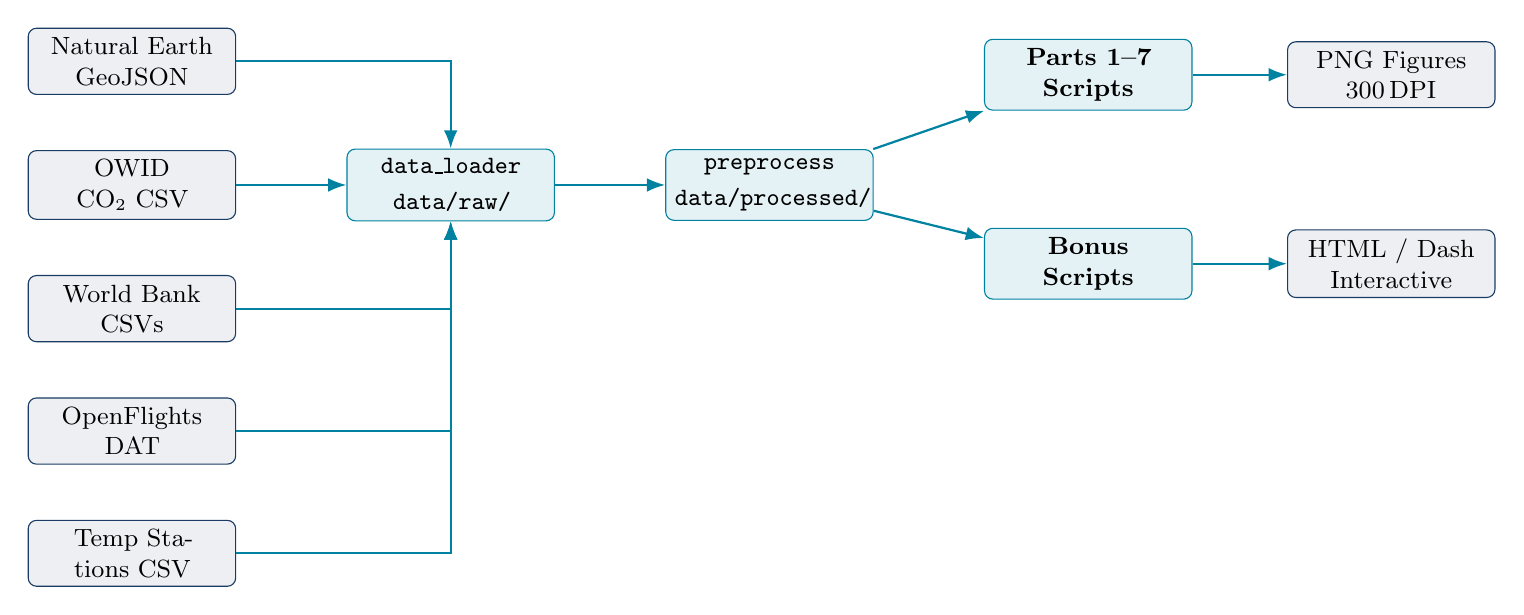
\begin{tikzpicture}[
    node distance = 0.7cm and 1.2cm,
    box/.style  = {draw=primary, rounded corners=3pt, fill=primary!8,
                   text width=2.4cm, align=center, font=\small},
    proc/.style = {draw=accent, rounded corners=3pt, fill=accent!10,
                   text width=2.4cm, align=center, font=\small\bfseries},
    arr/.style  = {-Latex, thick, color=accent},
  ]
    \node[box]               (ne)   {Natural Earth GeoJSON};
    \node[box, below=of ne]  (owid) {OWID CO\textsubscript{2} CSV};
    \node[box, below=of owid](wb)   {World Bank CSVs};
    \node[box, below=of wb]  (of)   {OpenFlights DAT};
    \node[box, below=of of]  (tmp)  {Temp Stations CSV};

    \node[proc, right=1.4cm of owid](dl)
      {\texttt{data\_loader}\\[2pt]\texttt{data/raw/}};

    \node[proc, right=1.4cm of dl]  (pp)
      {\texttt{preprocess}\\[2pt]\texttt{data/processed/}};

    \node[proc, right=1.4cm of pp, yshift= 1.4cm](p1){Parts 1--7\\Scripts};
    \node[proc, right=1.4cm of pp, yshift=-1.0cm](bn){Bonus\\Scripts};

    \node[box, right=1.2cm of p1](fig){PNG Figures\\300\,DPI};
    \node[box, right=1.2cm of bn](htm){HTML / Dash\\Interactive};

    \draw[arr] (ne)   -| (dl);
    \draw[arr] (owid) -- (dl);
    \draw[arr] (wb)   -| (dl);
    \draw[arr] (of)   -| (dl);
    \draw[arr] (tmp)  -| (dl);
    \draw[arr] (dl) -- (pp);
    \draw[arr] (pp) -- (p1);
    \draw[arr] (pp) -- (bn);
    \draw[arr] (p1) -- (fig);
    \draw[arr] (bn) -- (htm);
  \end{tikzpicture}%
  }
  \caption{End-to-end data-flow from external sources through processing to PNG figures
           and interactive HTML outputs. All intermediate artefacts live in
           \texttt{data/processed/}.}
  \label{fig:workflow}
\end{figure}

\section{Joins and Preprocessing}

The master GeoPackage \texttt{master\_world.gpkg} is assembled in
\texttt{scripts/utils/preprocess.py} through sequential left-joins:

\begin{enumerate}[leftmargin=2em, label=\textcolor{accent}{\bfseries Step~\arabic*:}]
  \item Natural Earth polygons $\leftarrow$ OWID CO\textsubscript{2} table
        (join key: ISO\,A3 country code).
  \item Result $\leftarrow$ World Bank population table
        (join key: country name / ISO code).
  \item Result $\leftarrow$ optional World Bank GDP / migration
        (join key: ISO code).
\end{enumerate}

Airport and route records are cleaned separately into \texttt{airports\_clean.csv} and
\texttt{routes\_clean.csv}, with coordinates validated and duplicate IATA codes removed.

% =============================================================
\chapter{Part~1 --- Projection Challenge}
% =============================================================

\begin{infobox}[Part~1 --- Core Question]
\textit{How does coordinate reference system (CRS) choice distort perceived area, shape,
and distance when mapping the same thematic variable globally?}
\end{infobox}

The same thematic variable --- \textbf{CO\textsubscript{2} emissions per capita} at the
analysis year set in \texttt{config.py} --- is rendered in three projections, each
preserving a different geometric property.

\section{Projections Compared}

\ts
\begin{table}[H]
  \centering
  \caption{Geometric properties preserved and distorted by each projection.}
  \label{tab:proj}
  \begin{tabularx}{\textwidth}{@{} L{2.5cm} Z Z Z @{}}
    \toprule
    \textbf{Projection} & \textbf{Preserves} & \textbf{Distorts} & \textbf{Best use} \\
    \midrule
    Albers Equal-Area        & Area                & Shape at extremes       & Area comparisons \\
    Lambert Conformal Conic  & Local angles/shape  & Area at high latitudes  & Navigation, regional \\
    Winkel Tripel            & Compromise balance  & Neither fully           & World reference maps \\
    \bottomrule
  \end{tabularx}
\end{table}

\section{Map Outputs}

\begin{figure}[H]
  \centering
  
\includegraphics[width=0.90\textwidth]{part1_projections/map_albers_equal_area.png}
  \caption{CO\textsubscript{2} per capita in \textbf{Albers Equal-Area}. Relative
           country areas are preserved, enabling a fair visual comparison of emission
           magnitudes. Shape distortion increases near the poles.}
  \label{fig:albers}
\end{figure}

\begin{figure}[H]
  \centering
  
\includegraphics[width=0.90\textwidth]{part1_projections/map_lambert_conformal.png}
  \caption{Same variable in \textbf{Lambert Conformal Conic}. Coastal outlines are
           locally accurate (shape preserved), but area comparisons between tropical
           and polar countries are unreliable.}
  \label{fig:lambert}
\end{figure}

\begin{figure}[H]
  \centering
  
\includegraphics[width=0.90\textwidth]{part1_projections/map_winkel_tripel.png}
  \caption{\textbf{Winkel Tripel} compromise projection, used by the National Geographic
           Society for world reference maps. Overall distortion is minimised; neither
           area nor shape is perfectly preserved.}
  \label{fig:winkel}
\end{figure}

\section{Key Finding}

\begin{designbox}
\textbf{Projection is not a cosmetic setting.} Switching from Albers to Lambert inflates
the visual footprint of Canada and Russia by a factor that can exceed $2\times$, directly
influencing which countries \emph{appear} to be the dominant emitters when pixel area
drives perceptual weight. Quantitative findings are recorded in\\
\texttt{outputs/figures/part1\_projections/projection\_comparison\_table.csv}.
\end{designbox}

% =============================================================
\chapter{Part~2 --- Choropleth Mapping and Pitfalls}
% =============================================================

\begin{infobox}[Part~2 --- Core Question]
\textit{How do classification scheme and variable normalisation change the story a choropleth
tells, and how can a choropleth mislead?}
\end{infobox}

\section{Classification Schemes}

Three schemes are applied to CO\textsubscript{2} \emph{per capita}:

\begin{enumerate}[leftmargin=2em, label=\textcolor{accent}{\bfseries\arabic*.}]
  \item \textbf{Quantiles} --- equal observation counts per class; reveals rank
        distribution but can merge very different values into the same class.
  \item \textbf{Natural Breaks (Jenks)} --- minimises within-class variance; best
        exposes natural groupings but class boundaries shift across datasets.
  \item \textbf{Equal Interval} --- fixed-width bins; arithmetically intuitive but
        produces near-empty classes when data are skewed.
\end{enumerate}

\begin{figure}[H]
  \centering
  
\includegraphics[width=\textwidth]{part2_choropleth/four_classification_schemes.png}
  \caption{Four-panel comparison of choropleth classification schemes applied to
           CO\textsubscript{2} per capita. Quantiles and Jenks natural breaks produce
           markedly different country groupings from identical underlying data.}
  \label{fig:fourclass}
\end{figure}

\begin{figure}[H]
  \centering
  
\includegraphics[width=0.88\textwidth]{part2_choropleth/map_quantiles.png}
  \caption{Quantile choropleth of CO\textsubscript{2} per capita (five classes). Each
           class holds the same number of countries; high-emitting outliers are
           absorbed into the top quintile without visual distinction.}
  \label{fig:quantiles}
\end{figure}

\section{Normalisation Critique}

A side-by-side figure contrasts \emph{total CO\textsubscript{2}} (raw count) against
\emph{CO\textsubscript{2} per capita}. China and the USA dominate the former; Qatar,
Kuwait, and Australia dominate the latter --- two entirely different narratives drawn
from the same emission records.

\section{Large-Area Visual Bias}

Russia, Canada, and Australia occupy disproportionate pixel area at common map scales,
causing viewers to over-estimate their contribution even when their per-capita values
are moderate. This bias is annotated in \texttt{part2\_choropleth/map\_area\_bias.png}
and discussed in \texttt{part2\_critique.txt}.

\begin{limitbox}
\textbf{Limitations:}
(i)~Missing data for small states creates visual gaps that may be misread as zero.
(ii)~All choropleth schemes impose discrete boundaries on continuous distributions.
(iii)~Colour-blind-unsafe palettes can invert the perceived ordering of classes.
\end{limitbox}

% =============================================================
\chapter{Part~3 --- Proportional Symbol Map}
% =============================================================

\begin{infobox}[Part~3 --- Core Question]
\textit{When a phenomenon is located at a point rather than spread across a polygon, how
should symbol size be scaled, and how can overplotting be managed?}
\end{infobox}

\section{Data and Scaling}

Airport route counts from OpenFlights drive symbol size. Two conventions are compared
in \texttt{part3\_comparison.txt}:

\begin{itemize}[leftmargin=2em]
  \item \textbf{Radius scaling} ($r \propto x$) --- overemphasises large airports; a
        hub with twice the routes appears four times larger in area.
  \item \textbf{Area scaling} ($r \propto \sqrt{x}$) --- perceptually correct; selected
        for the final map following Flannery's (1971) recommendations.
\end{itemize}

\begin{figure}[H]
  \centering
  
\includegraphics[width=0.90\textwidth]{part3_proportional/map_proportional_static.png}
  \caption{Proportional symbol map of global airport connectivity. Circle area is
           proportional to outbound route count (area scaling). Robinson projection;
           transparency ($\alpha = 0.55$) reduces overplotting at dense European and
           East Asian hubs.}
  \label{fig:prop}
\end{figure}

\section{Interactive Complement}

A Folium HTML map (\texttt{outputs/interactive/part3\_proportional\_folium.html}) enables
pan-and-zoom inspection of individual airports that overlap in the static figure. Click
popups display IATA code, city, country, and route count.

\begin{designbox}
\textbf{Design choice:} Robinson was selected over Mercator because it provides a less
distorted world view at global scale, avoiding the exaggerated Arctic band that would
inflate apparent symbol density at northern latitudes on a Mercator base.
\end{designbox}

% =============================================================
\chapter{Part~4 --- Flow Map and Network Analysis}
% =============================================================

\begin{infobox}[Part~4 --- Core Question]
\textit{Which country-pairs dominate global air traffic, and what network-theoretic
metrics characterise the airline hub structure?}
\end{infobox}

\section{Flow Construction}

OpenFlights routes are aggregated to \emph{country-pair} level (directed
origin--destination). Line width is proportional to route count; only the top flows
(threshold set in \texttt{config.py}) are drawn to avoid an illegible hairball.

\begin{figure}[H]
  \centering
  
\includegraphics[width=0.92\textwidth]{part4_flow/map_flow_routes.png}
  \caption{Flow map of the busiest country-pair airline corridors. Line width encodes
           normalised route count; colour hue distinguishes outbound from inbound
           balance. The USA--Europe and intra-Asia corridors dominate.}
  \label{fig:flow}
\end{figure}

\section{Network Analysis via NetworkX}

\ts
\begin{table}[H]
  \centering
  \caption{Network hub metrics for the top-10 countries by out-degree centrality.
           Values are populated after running \texttt{part4\_flow.py};
           see \texttt{network\_summary\_table.csv}.}
  \label{tab:network}
  \begin{tabularx}{\textwidth}{@{} L{2.5cm} >{\centering\arraybackslash}X >{\centering\arraybackslash}X >{\centering\arraybackslash}X >{\centering\arraybackslash}X @{}}
    \toprule
    \textbf{Country} & \textbf{Out-degree} & \textbf{In-degree} &
    \textbf{PageRank} & \textbf{Betweenness} \\
    \midrule
    \multicolumn{5}{c}{\small\itshape
      (Run \texttt{python run\_all.py --parts 4} to populate)} \\
    \bottomrule
  \end{tabularx}
\end{table}

\begin{limitbox}
\textbf{Limitations:} OpenFlights is volunteer-maintained and may omit regional carriers
or low-cost routes. Aggregating to country level discards airport-level geography.
Great-circle arcs are drawn straight in projected space; actual flight paths differ.
\end{limitbox}

% =============================================================
\chapter{Part~5 --- Continuous Field Mapping}
% =============================================================

\begin{infobox}[Part~5 --- Core Question]
\textit{How can sparse point measurements of temperature be interpolated into a smooth
surface, and what assumptions does this require?}
\end{infobox}

\section{Interpolation Methods}

Two methods are toggled via \texttt{config.py}:

\begin{itemize}[leftmargin=2em, label=\textcolor{accent}{\textbullet}]
  \item \textbf{Inverse Distance Weighting (IDW)} --- simple and fast; overfits near
        dense clusters, producing characteristic bull's-eye artefacts.
  \item \textbf{Radial Basis Function (RBF)} --- smoother surface; sensitive to the
        kernel function and smoothing parameter.
\end{itemize}

\begin{figure}[H]
  \centering
  
\includegraphics[width=0.86\textwidth]{part5_contour/map_temperature_points.png}
  \caption{Raw temperature station locations coloured by mean annual temperature.
           Spatial clustering over North America and Europe is evident; coverage gaps
           persist over ocean interiors and Antarctica.}
  \label{fig:temppts}
\end{figure}

\begin{figure}[H]
  \centering
  
\includegraphics[width=0.86\textwidth]{part5_contour/map_temperature_contour.png}
  \caption{Interpolated temperature surface with isopleth contours (diverging colour
           ramp centred at 10\textdegree{}C). Hatched regions indicate where station
           density is insufficient to justify interpolation confidence.}
  \label{fig:contour}
\end{figure}

\begin{designbox}
\textbf{Key assumptions:}
(i)~Temperature varies smoothly between stations --- violated over mountain ranges and
major ocean currents.
(ii)~The coordinate system is treated as locally Euclidean for the interpolation grid,
introducing error at high latitudes.
(iii)~Mean annual temperature collapses all seasonal variation into a single value.
\end{designbox}

% =============================================================
\chapter{Part~6 --- Cartogram and Area Correction}
% =============================================================

\begin{infobox}[Part~6 --- Core Question]
\textit{When geographic area dominates visual perception but is analytically irrelevant,
how can a cartogram correct the bias?}
\end{infobox}

\section{Standard Map versus Dorling Cartogram}

A standard geographic choropleth is paired with a \textbf{Dorling cartogram} in which
each country is replaced by a non-overlapping circle whose area encodes a chosen variable
(population or CO\textsubscript{2} total). This divorces visual weight from physical
territory.

\begin{figure}[H]
  \centering
  \begin{subfigure}[t]{0.47\textwidth}
    \centering
    
\includegraphics[width=\textwidth]{part6_cartogram/map_standard_geographic.png}
    \caption{Standard geographic map. Russia and Canada dominate visual space despite
             moderate per-capita emissions.}
    \label{fig:stdgeo}
  \end{subfigure}
  \hfill
  \begin{subfigure}[t]{0.47\textwidth}
    \centering
    
\includegraphics[width=\textwidth]{part6_cartogram/map_dorling_cartogram.png}
    \caption{Dorling cartogram: circle area $\propto$ population. Asia's demographic
             weight becomes immediately apparent.}
    \label{fig:dorling}
  \end{subfigure}
  \caption{Side-by-side comparison of the standard geographic map and the Dorling
           cartogram. The cartogram eliminates land-area dominance as a visual confound.}
  \label{fig:cartogram}
\end{figure}

\begin{limitbox}
\textbf{Limitations:} Dorling cartograms sacrifice spatial topology --- neighbouring
countries may no longer appear adjacent, which can disorient unfamiliar readers.
Clear labels are essential. The non-overlapping placement algorithm is stochastic;
repeated runs may produce slightly different circle arrangements.
\end{limitbox}

% =============================================================
\chapter{Part~7 --- Scenario-Based Map Design}
% =============================================================

\begin{infobox}[Part~7 --- Core Question]
\textit{How should map design --- layer selection, classification, colour, and symbology ---
be tailored to the decision context of the intended audience?}
\end{infobox}

Three applied scenarios are designed with documented rationale in
\texttt{part7\_design\_decisions.txt}.

\section{Scenario~A --- Public Health Risk}

\begin{figure}[H]
  \centering
  
\includegraphics[width=0.82\textwidth]{part7_scenarios/scenario_a_public_health.png}
  \caption{\textbf{Scenario A: Public health risk.} Choropleth of a health-vulnerability
           index overlaid with proportional symbols for hospital capacity. Sequential red
           ramp emphasises severity; symbol size encodes healthcare access deficit.
           Intended audience: policy-makers allocating emergency health resources.}
  \label{fig:scenA}
\end{figure}

\begin{designbox}
\textbf{Design rationale:} Red is culturally associated with danger in the target context.
Natural breaks classification avoids disguising low-risk countries as moderate-risk.
Hospital symbols are held as a separate layer to prevent conflating two distinct variables
into a single ambiguous encoding.
\end{designbox}

\section{Scenario~B --- Urban Service Accessibility}

\begin{figure}[H]
  \centering
  
\includegraphics[width=0.82\textwidth]{part7_scenarios/scenario_b_urban_services.png}
  \caption{\textbf{Scenario B: Urban service accessibility.} Multi-layer map combining
           administrative boundaries, transport network buffers, and point symbols for
           service facilities. Intended audience: urban planners identifying coverage gaps.}
  \label{fig:scenB}
\end{figure}

\section{Scenario~C --- Climate Risk Index}

\begin{figure}[H]
  \centering
  
\includegraphics[width=0.82\textwidth]{part7_scenarios/scenario_c_climate_risk.png}
  \caption{\textbf{Scenario C: Climate risk index.} Bivariate encoding combines
           CO\textsubscript{2} exposure (hue) with adaptive capacity (lightness),
           producing a $3{\times}3$ legend matrix. Countries with high exposure
           \emph{and} low capacity occupy the darkest, most saturated cells.
           Intended audience: climate finance institutions.}
  \label{fig:scenC}
\end{figure}

% =============================================================
\chapter{Bonus --- Interactive Outputs and Spatial Statistics}
% =============================================================

Optional extensions beyond the core seven parts.

\section{Plotly Dash Dashboard}

\texttt{scripts/bonus/bonus\_dashboard.py} launches an interactive dashboard on
port~8050 with a year-slider over the CO\textsubscript{2} choropleth, a country-detail
panel, and an airline network sub-graph viewer. It is excluded from \texttt{run\_all.py}
because it blocks the terminal with a live server process.

\section{Temporal Choropleth Animation}

\texttt{bonus\_animation.py} builds a Plotly HTML animation.
Frames cover 1990 through the analysis year in \texttt{config.py}.
Output: \url{outputs/interactive/animations/co2_animation.html}.

\section{Moran's\,I and LISA Spatial Autocorrelation}

\texttt{bonus\_morans\_i.py} (PySAL / \texttt{esda} package) computes:

\begin{itemize}[leftmargin=2em, label=\textcolor{accent}{\textbullet}]
  \item \textbf{Global Moran's\,I} for CO\textsubscript{2} per capita --- tests whether
        high-emitting countries cluster spatially rather than disperse randomly.
  \item \textbf{LISA} (Local Indicators of Spatial Association) --- identifies
        High--High, Low--Low, High--Low, and Low--High outlier clusters at country level.
\end{itemize}

Results and significance maps are saved to
\texttt{outputs/figures/bonus\_morans/}.

% =============================================================
\chapter{Reproducibility and Pipeline Management}
% =============================================================

\section{Configuration System}

All tunable parameters are centralised in \texttt{config.py} (under \texttt{scripts/utils/}).
To regenerate figures, change \texttt{ANALYSIS\_YEAR} or \texttt{DPI\_FINAL} and run
\texttt{run\_all.py}; no edits to the part-scripts are required.

\begin{lstlisting}[
  language=Python,
  caption={Key configuration constants in \texttt{config.py}.},
  label={lst:config},
  basicstyle=\ttfamily\footnotesize,
]
# --- Analysis parameters ---
ANALYSIS_YEAR    = 2020

# --- Directory paths ---
RAW_DIR          = Path("data/raw")
PROCESSED_DIR    = Path("data/processed")
FIGURES_DIR      = Path("outputs/figures")
INTERACTIVE_DIR  = Path("outputs/interactive")

# --- Figure quality ---
DPI_FINAL        = 300
DPI_DRAFT        = 150
DEFAULT_FIG_SIZE = (14, 8)    # inches (width, height)

# --- CRS strings (split for line width; equivalent single-line strings in repo) ---
CRS_ALBERS       = (
    "+proj=aea +lat_1=29.5 +lat_2=45.5 +lon_0=0"
)
CRS_LAMBERT      = (
    "+proj=lcc +lat_1=33 +lat_2=45 +lon_0=0"
)
CRS_WINKEL       = "+proj=wintri"
CRS_ROBINSON     = "+proj=robin +lon_0=0"
CRS_GEOGRAPHIC   = "EPSG:4326"
\end{lstlisting}

\section{Pipeline Commands}

\footnotesize
\ts
\begin{table}[H]
  \centering
  \caption{Orchestration commands for the full pipeline.}
  \label{tab:commands}
  \begin{tabularx}{\textwidth}{@{} >{\ttfamily\raggedright\arraybackslash}p{0.46\textwidth} Z @{}}
    \toprule
    \textbf{Command} & \textbf{Purpose} \\
    \midrule
    \texttt{python scripts/utils/data\_loader.py}
      & Download all raw source files \\
    \texttt{python scripts/utils/preprocess.py}
      & Build \texttt{data/processed/} \\
    \texttt{python run\_all.py}
      & Full pipeline, parts 1--7 at 300\,DPI \\
    \texttt{python run\_all.py --draft}
      & Same at 150\,DPI for rapid iteration \\
    \texttt{python run\_all.py --parts 1 2 3}
      & Selected parts only \\
    \texttt{python run\_all.py --skip-download}
      & Regenerate figures, skip download \\
    \texttt{python run\_all.py --bonus --skip-download}
      & Batch bonus HTML outputs only \\
    \texttt{python scripts/bonus/bonus\_dashboard.py}
      & Launch live Dash server (port 8050) \\
    \texttt{pytest tests/ -v}
      & Run automated test suite \\
    \bottomrule
  \end{tabularx}
\end{table}
\normalsize

% =============================================================
\chapter{Conclusion}
% =============================================================

This portfolio demonstrates that \textbf{map choice and classification shape analytical
narrative} as powerfully as the underlying data. The key lessons from the seven parts
are as follows.

\begin{enumerate}[leftmargin=2em, label=\textcolor{accent}{\bfseries\arabic*.}]
  \item \textbf{Projections are analytical decisions,} not cosmetic ones. Equal-area
        projections are obligatory whenever visual area comparisons are intended.
  \item \textbf{Choropleth classification is rhetorical.} The same data tells
        dramatically different stories under quantile versus equal-interval schemes;
        per-capita normalisation is almost always required.
  \item \textbf{Proportional symbols belong at points.} Placing them on polygon
        centroids conflates the symbol's apparent location with the polygon's extent.
  \item \textbf{Flow maps require ruthless filtering.} Rendering all routes produces
        illegible hairballs; only dominant corridors convey meaningful structure.
  \item \textbf{Continuous-field interpolation assumes smooth variation.} Invalid
        assumptions over mountain ranges or ocean boundaries must be disclosed.
  \item \textbf{Cartograms counter land-area dominance.} They trade geographic
        familiarity for analytical accuracy and always require clear labels.
  \item \textbf{Scenario design is audience-driven.} Colour, classification, and layer
        selection must reflect the decision context, not personal aesthetic preference.
\end{enumerate}

All limitations are recorded in the generated \texttt{.txt} files alongside the
corresponding figures, fulfilling the requirement for transparent, self-critiquing
analysis.

% =============================================================
%  REFERENCES
% =============================================================
\clearpage
\addcontentsline{toc}{chapter}{References}
\begin{thebibliography}{99}

\bibitem{naturalearth}
Natural Earth (2023).
\textit{Admin 0 --- Countries, 110m cultural vectors.}
Public Domain.
\url{https://www.naturalearthdata.com/}

\bibitem{owid}
Our World in Data (2023).
\textit{CO\textsubscript{2} and greenhouse gas emissions.}
CC~BY~4.0.
\url{https://ourworldindata.org/co2-and-greenhouse-gas-emissions}

\bibitem{openflights}
OpenFlights (2023).
\textit{Airport and route database.}
Open Database Licence (ODbL).
\url{https://openflights.org/data.html}

\bibitem{worldbank}
World Bank (2023).
\textit{Population totals and GDP per capita.}
CC~BY~4.0.
\url{https://data.worldbank.org/}

\bibitem{geopandas}
Jordahl,~K.\ et~al.\ (2023).
\textit{GeoPandas: Python tools for geographic data.}
\url{https://geopandas.org/}

\bibitem{mapclassify}
Rey,~S.\,J., Anselin,~L., et~al.\ (2023).
\textit{mapclassify: Classification schemes for choropleth maps.}
\url{https://pysal.org/mapclassify/}

\bibitem{folium}
Filipe,~R.\ et~al.\ (2023).
\textit{Folium: Python data, Leaflet.js maps.}
\url{https://python-visualization.github.io/folium/}

\bibitem{networkx}
Hagberg,~A.\,A., Schult,~D.\,A.,\ \& Swart,~P.\,J.\ (2008).
Exploring network structure, dynamics, and function using NetworkX\@.
\textit{Proceedings of the 7th Python in Science Conference}, pp.~11--15.

\bibitem{pysal}
Rey,~S.\,J.\ \& Anselin,~L.\ (2007).
PySAL: A Python library of spatial analytical methods.
\textit{The Review of Regional Studies}, 37(1), 5--27.

\bibitem{flannery}
Flannery,~J.\,J.\ (1971).
The relative merits of the circle and the bar as representations of component part
statistics.
\textit{The Canadian Cartographer}, 8(2), 96--109.

\end{thebibliography}

% =============================================================
%  APPENDICES
% =============================================================
\appendix
\chapter{Output File Manifest}
\label{app:manifest}

\footnotesize
\ts
\setlength{\tabcolsep}{4pt}
\begin{longtable}{@{} p{7.6cm} L{6.4cm} @{}}
  \caption{Expected files under \texttt{outputs/} after a full pipeline run.}
  \label{tab:manifest} \\
  \toprule
  \rowcolor{primary!10}
  \textbf{File path} & \textbf{Description} \\
  \midrule
  \endfirsthead
  \multicolumn{2}{c}{\small\itshape (Table continued)} \\
  \toprule
  \rowcolor{primary!10}
  \textbf{File path} & \textbf{Description} \\
  \midrule
  \endhead
  \bottomrule
  \endfoot
  \bottomrule
  \endlastfoot

  \url{figures/part1_projections/map_albers_equal_area.png}  & Part 1, Albers \\
  \url{figures/part1_projections/map_lambert_conformal.png}   & Part 1, Lambert \\
  \url{figures/part1_projections/map_winkel_tripel.png}       & Part 1, Winkel Tripel \\
  \url{figures/part1_projections/projection_comparison_table.csv} & Part 1 data table \\
  \rowcolor{lightgray}
  \url{figures/part2_choropleth/map_quantiles.png}             & Part 2, quantile scheme \\
  \rowcolor{lightgray}
  \url{figures/part2_choropleth/four_classification_schemes.png} & Part 2, four-panel \\
  \rowcolor{lightgray}
  \url{figures/part2_choropleth/large_area_bias_annotated.png} & Part 2, area-bias annotation \\
  \url{figures/part3_proportional/map_proportional_static.png} & Part 3, static \\
  \url{interactive/part3_proportional_folium.html}             & Part 3, Folium HTML \\
  \rowcolor{lightgray}
  \url{figures/part4_flow/map_flow_routes.png}                & Part 4, flow map \\
  \rowcolor{lightgray}
  \url{figures/part4_flow/network_summary_table.csv}          & Part 4, NetworkX metrics \\
  \url{figures/part5_contour/map_temperature_points.png}      & Part 5, station points \\
  \url{figures/part5_contour/map_temperature_contour.png}     & Part 5, isopleth surface \\
  \rowcolor{lightgray}
  \url{figures/part6_cartogram/map_standard_geographic.png}   & Part 6, geographic \\
  \rowcolor{lightgray}
  \url{figures/part6_cartogram/map_dorling_cartogram.png}     & Part 6, Dorling \\
  \url{figures/part7_scenarios/scenario_a_public_health.png} & Part 7, Scenario A \\
  \url{figures/part7_scenarios/scenario_b_urban_services.png}& Part 7, Scenario B \\
  \url{figures/part7_scenarios/scenario_c_climate_risk.png}  & Part 7, Scenario C \\
  \rowcolor{lightgray}
  \url{interactive/animations/co2_animation.html}               & Bonus, temporal animation \\
  \rowcolor{lightgray}
  \url{figures/bonus_morans/moran_scatter.png}                 & Bonus, Moran's~I \\
  \rowcolor{lightgray}
  \url{figures/bonus_morans/lisa_map.png}                      & Bonus, LISA clusters \\
\end{longtable}
\setlength{\tabcolsep}{6pt}
\normalsize

% ── Appendix B ───────────────────────────────────────────────
\chapter{Compilation Instructions}
\label{app:compile}

\begin{figure}[H]
  \centering
  \begin{BVerbatim}[fontsize=\small]
# --- Step 1: generate all figures (from repo root) ---
python run_all.py

# --- Step 2: compile the report (from the report/ folder) ---
#   Run pdflatex TWICE (TOC and cross-references).
cd report/
pdflatex GeoMetric-Report.tex
pdflatex GeoMetric-Report.tex

# --- Alternative A: Pandoc / build script ---
python scripts/build_report_pdf.py

# --- Alternative B: HTML then print to PDF ---
python scripts/build_report_pdf.py --html
  \end{BVerbatim}
  \caption{Commands to generate all figures and compile this report to PDF.}
  \label{fig:compilecmds}
\end{figure}

\begin{limitbox}
\textbf{Important:} If any \verb|\includegraphics| reports ``File not found'', verify
that \texttt{outputs/figures/} exists and that \texttt{python run\_all.py} completed
without errors \emph{before} compiling. The \verb|\graphicspath| declaration searches
\texttt{../outputs/figures/} (correct when compiling from \texttt{report/}),
\texttt{outputs/figures/} (correct from repo root), and \texttt{./} (if PNG files are
placed in the same folder as this \texttt{.tex} file).
\end{limitbox}

\end{document}